\documentclass[12pt]{article}
%\usepackage[english]{babel}
%\usepackage[utf8x]{inputenc}
%\usepackage{amsmath}
\usepackage{tikz}
\usetikzlibrary{arrows,automata}
\begin{document}
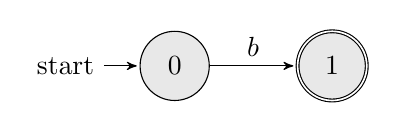
\begin{tikzpicture}[->,>=stealth',shorten >=1pt,auto,node distance=2cm,
        scale = 1,transform shape]
        \tikzstyle{every state}=[fill={rgb:black,1;white,10}]
  \node[state,initial] (0) {$0$};
  \node[state,accepting] (1) [right of=0] {$1$};

  \path (0) edge              node {$b$} (1);

\end{tikzpicture}
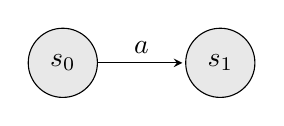
\begin{tikzpicture}[->,>=stealth,shorten >=1pt,node distance=2cm,auto,
    scale = 1,transform shape]
    \tikzstyle{every state}=[fill={rgb:black,1;white,10}]
  
    \node[state] (0) {$s_0$};
    \node[state] (1) [right of=0] {$s_1$};
    \path
    (0) edge[above]  node{$a$} (1);

  \end{tikzpicture}
\end{document}
